\chapter{Randomness}
\begin{flushleft}
    I protocolli di crittografia sono spesso basati su \textbf{generatori di dati random}, ad esempio per la generazione delle \textbf{chiavi} o dell'\textbf{IV}. È importante differenziare un valore random con un valore \textbf{crittograficamente randomico} ovvero dati \textbf{impredicibili} che possono essere campionati da una distribuzione uniforme o coinvolgere altre tipologie di distribuzione - ad esempio quella Gaussiana. \\
    Molti eventi del mondo reale sono noti - nella fisica - come governati  da:
    \begin{itemize}[nosep]
        \item eventi probabilistici che sono ``realmente'' casuali o imprevedibili, ad esempio quelli studiati dalla fisica quantistica.
        \item comportamenti deterministici che sono molto difficili da prevedere in quanti gli output sono molto sensibili anche a variazioni molto piccole degli input, normalmente studiati nella teoria del caos.
    \end{itemize}

    \smallskip

    \textcolor{red}{\textbf{Entropia}}: in ambito crittografico rappresenta l'imprevedibilità di un'informazione, maggiore è l'entropia, più è difficile per un attaccante indovinare o ricostruire quel dato. Ad esempio consideriamo una chiave a 128bit generata partendo da una scelta casuale di un solo bit attraverso un algoritmo deterministico, a quel punto avremo che la lunghezza della chiave sarà 128bit, ma i suoi bit di entropia sarà soltanto uno e questo fatto la rende facilmente attaccabile. \\
    Normalmente in crittografia si richiede che la chiave abbia $n$ bit di \textbf{entropia}, ovvero il nostro spazio delle chiavi sarà formato da $2^n$ tutti \textbf{equiprobabili}. Queste congettura, tuttavia, non valgono per \textbf{password} o \textbf{PIN}.

    \smallskip

    Consideriamo \textbf{chiavi crittografiche segrete uniformemente casuali} su stringhe binarie: in questo caso la lunghezza in bit è pari all'entropia della chiave. Nel caso di \textbf{PIN} avremo una sequenza di $n$ numeri, possiamo calcolare la probabilita che esca un determinato numero: $\log_2(10^n)$ - ad esempio per $n = 4$ avremo che i bit di entropia saranno $\log_2(10^4) \simeq 13.28$bit. Invece, per una \textbf{password}, dipende dall'alfabeto scelto ($n$) - quindi la sua cardinalità - e dalla lunghezza della password ($N$), il calcolo dei bit di entropia sarà: $N \times \log_2(10^n)$. Nel caso di \textbf{password} il reale livello di sicurezza è molto più basso in quanto il campionamento dei simboli non è sempre uniforme all'interno del loro dominio o indipendentemente l'uno dall'altro. Infatti difficilmente la mente umana è capace di ricordarsi dati completamente random e quindi la sicurezza di una password di dimensione $N$ è molto inferiore alla precendente stima.

    \smallskip

    Considerando applicativi su cui è necessario far girare algoritmi di crittografia, e considerando che tali applicativi sono software, per ottenere un dato random ``buono'' non possiamo affidarci ad un computer in quanto sono intrinsecamente \textbf{deterministici} e \textbf{predicibili} è quindi necessario fare affidamente su \textbf{fonti esterne} che sono associate a dati intrinsecamente randomici o eventi fisici impredicibili (camere, input dell'utente, \textit{interrupt hardware}). Esisto degli hardware dedicati, chiamati: \textbf{\textit{True Random Number Generator - TRNG}} che venono alimentati da eventi fisici (\textit{thermal noise}) che vengono quindi utilizzati come fonti esterne di bit random (molto utili per server e sistemi embedded), queste sorgenti esterne vengono spesso identificate come \textbf{\textit{noise source}}
    
    \smallskip

    Le \textbf{sorgenti di entropia} vengono prima processate dal sistema operativo prima di essere rese disponibili ad altri servizi. Questo permette di ottenere fonti di entropia miste:
    \begin{itemize}[nosep]
        \item aumento di ``fiducia'' nella qualità dei dati casuali.
        \item mitigare potenziali rischi di attacchi alle fonti.
        \item ridurre i rischi relativi alle fonti di \textbf{backdoor}
    \end{itemize}
    Inoltre permette anche di espandere i ``veri'' dati casuali per aumentare la disponibilità di dati ad alta entropia.

    \begin{figure}[h]
        \centering
        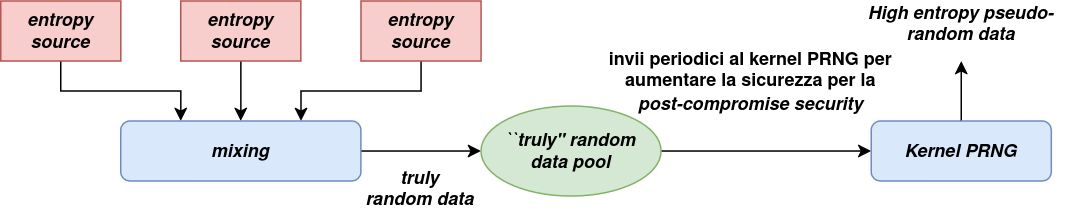
\includegraphics[width=0.75\textwidth]{img/prng_pool.png}
    \end{figure}

    Il lavoro del \textbf{\textit{Kernel PRNG}} è simile a quello di uno \textit{stream cipher} ma il suo schematico è leggermente differente in quanto vi è una modellazione dell'avversario diversa. Che permette di aumentare la sicurezza attraverso lo sviuppo di mitigazioni contro a \textbf{compromissioni non permanenti}:
    \begin{itemize}[nosep]
        \item \textbf{\textit{forward secrecy}}: se l'avversario compromette il sistema in un istante di tempo $t_i$ non dovrà riuscire ad ottenere informazioni su istanti di tempo $t_k$ con $k < i$, per ottenere questa garanzia si possono utilizzare delle funzioni \textbf{\textit{one-way}} - ad esempio le \textit{hash function}.
        \item \textbf{\textit{post-compromise security}}: è duale alla \textit{forward secrecy} ovvero che se l'avversario compromette il sistema in un istante $t_i$ non dovrà riuscire ad ottenere stati futuri in maniera deterministica.
    \end{itemize}
    Queste due proprietà (\textbf{\textit{Security Guarantees}}) vanno a descrivere un attaccante che non deve essere capace di creare persistenza nel sistema.

    \smallskip

    \textbf{\textit{Kernel vs. User space}}, in passato molte librerie crittografiche non si fidavano della routine del sistema operativo per generare numeri casuali sicuri, infatti si credeva che il \textbf{kernel} avesse una \textbf{PRNG} debole venne quindi adottata una soluzione, ovvero le librerie crittografiche \textbf{implementavano} un priorio \textit{PRNG custom} in \textbf{\textit{user space}} - chiamato anche \textbf{\textit{userland PRNG}}, ma veniva spesso sbagliata l'impementazione e questi dati avere un entropia molto bassa. Un esempio famoso fu nel 2008 che debian, dopo una modifica al codice sorgente rese prevedibile la generazione della chiave private ssh. Oggigiorno ci si affida maggiormente al sistema operativo e alle API per la generazione di valori randomici.
    
    \smallskip

    Un altro problema molto importante era il \textbf{\textit{reesiding at fork}} infatti se non specificato, nel momento in cui veniva eseguita una \textbf{fork} e successivamente \textit{spawnato} un processo figlio se non veniva aggiornato il pool di entropia, sia il padre che il/i figli avrebbero generato la stessa sequenza di valore \textit{pseudo-random}.

    \smallskip

    \textbf{\textit{Virtual Machine Cloning}}: clonare una macchina virtuale poteva causare problemi al \textit{kernel PRNG} simili all'utilizzo di una \textbf{fork} questo comportava:
    \begin{itemize}[nosep]
        \item multi-VMs accese nello stesso istante generavano gli stessi pseudo-random data.
        \item la soluzione fu quella di re-inizializzare il pool durante l'avvio della VMs
    \end{itemize}

    \smallskip

    \textbf{\textit{Low entropy in early boot phases and embedded devices}} nelle fasi iniziali di boot, soprattuto nei dispositivi embedded, il pool potrebbe essere molto basso, se non inesistente questo comportava l'arresto o la generazione di pseudo-random deboli a seconda della strategia adottata - bloccante o attesa - la soluzione fu quella di adottare una \textbf{\textit{TRNG Hardware}}
\end{flushleft}